\documentclass[12pt,a4paper]{article}

\usepackage{polyglossia}
\setmainlanguage{english}
\setotherlanguage{hebrew}
\usepackage{fontspec}
\directlua{
  luaotfload.add_fallback("hebrewfallback", {
    "David CLM:mode=harf;script=hebr;"
  })
}
\setmainfont{Latin Modern Roman}[RawFeature={fallback=hebrewfallback}]
\newfontfamily\hebrewfont[Script=Hebrew]{David CLM}
\usepackage{luabidi}
\usepackage{geometry}
\geometry{margin=2.5cm}
\usepackage{setspace}
\onehalfspacing
\usepackage{titlesec}
\usepackage{hyperref}
\usepackage{biblatex}
\addbibresource{references.bib}
\usepackage{booktabs}
\usepackage{float}
\usepackage{amsmath}
\usepackage{array}
\usepackage{ragged2e}
\usepackage{tabularx}
\usepackage{caption}
\usepackage{tikz}
\usetikzlibrary{shapes,arrows.meta,positioning}
\usepackage{pgfplots}
\pgfplotsset{compat=1.18}
\usepackage{tcolorbox}
\tcbuselibrary{skins,breakable}
\newenvironment{hebrewblock}{%
  \begin{tcolorbox}[enhanced,breakable,parbox=false,
    colback=blue!4!white,colframe=blue!28!white,
    left=8pt,right=8pt,top=6pt,bottom=6pt,arc=2pt,boxrule=0.5pt]%
  \hebrewfont\begin{hebrew}%
}{%
  \end{hebrew}\end{tcolorbox}\vspace{3pt}%
}
\newenvironment{englishblock}{%
  \begin{tcolorbox}[enhanced,breakable,parbox=false,
    colback=gray!5!white,colframe=gray!28!white,
    left=8pt,right=8pt,top=6pt,bottom=6pt,arc=2pt,boxrule=0.5pt]%
  \normalfont\setLR%
}{%
  \end{tcolorbox}\vspace{3pt}%
}
\usepackage{graphicx}
\usepackage{fancyhdr}
\setlength{\headheight}{14pt}
\pagestyle{fancy}
\usepackage{todonotes}

\fancyhf{}
\fancyhead[L]{\leftmark}
\fancyhead[R]{\thepage}
\fancyfoot[C]{203.3763 --- Orchestration of AI Agents --- June 2026}
\renewcommand{\headrulewidth}{0.4pt}
\renewcommand{\footrulewidth}{0.4pt}

\begin{document}

\begin{titlepage}
  \thispagestyle{empty}
  \centering

  \includegraphics[width=5cm]{../assets/images/uniHaifasymbol.png}\par
  \vspace{0.4cm}

  {\large\bfseries University of Haifa\par}
  {\normalsize Department of Information Systems\par}

  \vspace{1.2cm}\hrule\vspace{1.2cm}

  {\Huge\bfseries AI Agents in Healthcare: Transforming Patient Care and Operational Efficiency\par}
  \vspace{0.3cm}
  {\Large\bfseries Ethical, Regulatory, and Technological Considerations for Responsible Integration\par}

  \vspace{0.5cm}
  {\hebrewfont\large
    \begin{hebrew}
      סוכני בינה מלאכותית בשירותי הבריאות: טרנספורמציה בטיפול בחולים וביעילות תפעולית
    \end{hebrew}\par}

  \vfill

  \begin{tabular}{rl}
    \textbf{Author:}    & Nagham Manasra \& Yaman Dahle \\[4pt]
    \textbf{Course:}     & 203.3763 --- Orchestration of AI Agents \\[4pt]
    \textbf{Instructor:} & Dr. Yoram Segal \\[4pt]
    \textbf{Date:}      & June 2026 \\
  \end{tabular}

  \vspace{1.2cm}\hrule\vspace{0.6cm}

  {\large June 2026\par}
\end{titlepage}

\newpage
\tableofcontents
\newpage

\begin{abstract}
Artificial Intelligence (AI) agents are rapidly emerging as transformative tools within the healthcare sector. This article explores their diverse applications, ranging from enhancing diagnostic accuracy to streamlining administrative workflows and personalizing treatment plans. The underlying technologies, including deep learning and natural language processing, enable these agents to process vast amounts of data and provide actionable insights. While AI agents offer unprecedented opportunities to revolutionize healthcare by augmenting human capabilities and improving operational efficiency, their successful and ethical integration hinges on robust regulatory frameworks, transparent algorithmic design, and a proactive approach to addressing inherent biases. Ensuring patient trust and accountability for errors are paramount for widespread adoption. This paper systematically examines the current landscape, identifies critical challenges, and offers forward-looking perspectives on the responsible development and deployment of AI agents in healthcare.
\end{abstract}

\section{Introduction to AI Agents in Healthcare}
The integration of Artificial Intelligence (AI) into healthcare represents a significant advancement, promising to reshape how medical services are delivered and managed \cite{topol2019deep}. AI agents, defined as autonomous or semi-autonomous systems capable of perceiving their environment and taking actions to achieve specific goals, are at the forefront of this transformation. These agents leverage sophisticated algorithms and vast datasets to perform tasks that traditionally required human cognitive effort, often with enhanced speed and precision \cite{russell2010artificial}. Their deployment across various medical domains signals a new era of augmented intelligence, where human expertise is amplified by computational power.

The purpose of this article is to explore the burgeoning field of AI agents within healthcare, focusing on their diverse applications, underlying technologies, and the complex interplay of ethical, regulatory, and practical challenges they present. It delves into how these systems are transforming patient care, diagnostics, and administrative processes, highlighting their potential to enhance efficiency and outcomes. This paper argues that while AI agents offer unprecedented opportunities to revolutionize healthcare, their successful and ethical integration hinges on robust regulatory frameworks, transparent algorithmic design, and a proactive approach to addressing inherent biases and ensuring patient trust. The subsequent sections will systematically address these aspects, providing a comprehensive overview of the current landscape and future directions.

\subsection{Defining AI Agents and Their Role}
AI agents are computational entities designed to act intelligently within a given environment. In healthcare, this means they can process clinical data, learn from patterns, and execute tasks such as diagnosis, treatment recommendation, or administrative automation \cite{goodfellow2016deep}. Their autonomy levels vary, ranging from decision support systems that assist clinicians to fully autonomous robotic surgical assistants. The primary role of these agents is to augment human capabilities, reduce workload, and improve the overall quality and accessibility of healthcare services.

The distinction between general AI systems and AI agents lies in their capacity for goal-directed action and interaction with their environment. AI agents are not merely analytical tools; they are designed to perform specific functions and often interact with other systems or human users. This active role necessitates careful consideration of their design, deployment, and oversight. Understanding these foundational concepts is crucial for appreciating the scope and impact of AI in modern medicine.

\subsection{Historical Context of AI in Medicine}
The application of AI in medicine is not a new concept, with early expert systems emerging in the 1970s and 1980s. These systems, such as MYCIN, aimed to diagnose infectious diseases and recommend treatments based on rule-based logic \cite{russell2010artificial}. While limited by computational power and data availability, they laid the groundwork for future advancements. The resurgence of AI, particularly with the advent of machine learning and deep learning, has dramatically expanded its potential in healthcare.

Modern AI agents benefit from massive datasets, advanced algorithms, and powerful computing infrastructure, enabling them to tackle complex problems previously intractable. This evolution from rule-based systems to data-driven models marks a significant paradigm shift. The historical trajectory demonstrates a continuous pursuit of intelligent automation and decision support in clinical practice, culminating in the sophisticated AI agents seen today.

\subsection{Scope and Relevance of AI Agents}
The scope of AI agents in healthcare is vast, encompassing clinical, operational, and research domains. Clinically, they assist in diagnostics, personalized treatment, and patient monitoring. Operationally, they streamline administrative tasks, optimize resource allocation, and enhance revenue cycle management. In research, they accelerate drug discovery and clinical trials \cite{davenport2019ai}.

The relevance of AI agents is underscored by the increasing demands on healthcare systems, including rising costs, workforce shortages, and the need for more personalized and preventive care. By automating routine tasks and providing advanced analytical capabilities, AI agents can improve efficiency, reduce errors, and ultimately enhance patient outcomes. Their ability to process and synthesize information at scale makes them indispensable tools for the future of medicine.

\section{Categorization and Functionalities of AI Agents}
AI agents in healthcare are diverse, categorized primarily by their level of autonomy and specific functionalities. This categorization helps in understanding their operational scope and the regulatory challenges associated with their deployment. From highly autonomous systems to those providing decision support, each type of agent plays a distinct role in the healthcare ecosystem. The spectrum of autonomy ranges from fully automated processes to human-in-the-loop systems that require clinician oversight.

Understanding these distinctions is crucial for effective implementation and for addressing the ethical and safety implications of AI in clinical practice. The classification also informs the development of appropriate validation and monitoring strategies. This section details the various types of AI agents and their primary functions within healthcare.

\subsection{Diagnostic Support Agents}
Diagnostic support agents are designed to assist clinicians in identifying diseases by analyzing medical images, patient symptoms, and laboratory results \cite{esteva2017dermatologist}. These agents often employ deep learning models to detect subtle patterns that might be missed by the human eye. For example, AI agents can analyze mammograms for early signs of breast cancer or retinal scans for diabetic retinopathy with high accuracy \cite{rajpurkar2017chexnet}. Their ability to process large volumes of data quickly enhances diagnostic speed and consistency.

These agents do not typically make final diagnoses independently but provide probabilities and highlight areas of concern for clinicians to review. This collaborative approach leverages the AI's analytical power while retaining human oversight. The goal is to reduce diagnostic errors and improve patient outcomes through early and accurate detection. The integration of such tools requires careful validation against human expert performance.

\subsection{Personalized Treatment Planning Agents}
Personalized treatment planning agents utilize extensive patient data, including genetic information, medical history, and lifestyle factors, to recommend tailored treatment strategies \cite{topol2019highperformance}. These agents can predict individual responses to different therapies, optimize drug dosages, and suggest preventive measures. They move beyond a one-size-fits-all approach, enabling precision medicine that is highly specific to each patient's unique biological profile.

By analyzing complex interactions between various patient parameters, these agents can identify optimal pathways for managing chronic diseases or selecting the most effective cancer therapies. This capability is particularly valuable in oncology, where treatment efficacy can vary significantly among individuals. The aim is to improve therapeutic outcomes and minimize adverse effects by customizing interventions. The system architecture for such agents often involves multiple interconnected modules, as illustrated in Figure \ref{fig:treatment_planning}.

\begin{figure}[H]
  \centering
  \begin{tikzpicture}[node distance=2cm, auto, >=Stealth]
    % Nodes
    \node (input) [rectangle, draw, fill=blue!10, text width=3cm, minimum height=1cm, text centered] {Data Input (EHR, Genomics, Lifestyle)};
    \node (preprocessing) [rectangle, draw, fill=green!10, text width=3cm, minimum height=1cm, text centered, below of=input, yshift=-0.5cm] {Data Preprocessing \& Feature Engineering};
    \node (mlmodel) [rectangle, draw, fill=orange!10, text width=3cm, minimum height=1cm, text centered, below of=preprocessing, yshift=-0.5cm] {ML Models (Deep Learning, Reinforcement Learning)};
    \node (risk) [rectangle, draw, fill=red!10, text width=3cm, minimum height=1cm, text centered, below of=mlmodel, yshift=-0.5cm] {Risk Assessment \& Outcome Prediction};
    \node (output) [rectangle, draw, fill=purple!10, text width=3cm, minimum height=1cm, text centered, below of=risk, yshift=-0.5cm] {Treatment Recommendations \& Alerts};
    \node (clinician) [rectangle, draw, fill=gray!10, text width=3cm, minimum height=1cm, text centered, right of=output, xshift=2.5cm] {Clinician Review \& Decision};

    % Edges
    \draw[->] (input) -- (preprocessing) node[midway, right, fill=white, inner sep=2pt, font=\footnotesize] {Raw Data};
    \draw[->] (preprocessing) -- (mlmodel) node[midway, right, fill=white, inner sep=2pt, font=\footnotesize] {Cleaned Features};
    \draw[->] (mlmodel) -- (risk) node[midway, right, fill=white, inner sep=2pt, font=\footnotesize] {Model Outputs};
    \draw[->] (risk) -- (output) node[midway, right, fill=white, inner sep=2pt, font=\footnotesize] {Actionable Insights};
    \draw[->] (output) -- (clinician) node[midway, above, fill=white, inner sep=2pt, font=\footnotesize] {Recommendations};
    \draw[->] (clinician) -- (input.east) node[midway, above, fill=white, inner sep=2pt, font=\footnotesize, xshift=0.5cm, yshift=1.5cm] {Feedback Loop};
  \end{tikzpicture}
  \caption{Architectural diagram illustrating a typical AI agent system for personalized treatment planning, showing data input, AI processing modules, and output \cite{ibm_watson_health}.}
  \label{fig:treatment_planning}
\end{figure}

\subsection{Administrative and Operational Agents}
Beyond direct patient care, AI agents significantly enhance administrative and operational efficiency within healthcare organizations. These agents automate routine tasks such as patient scheduling, billing, insurance verification, and electronic health record (EHR) management \cite{televox_patient_engagement}. By reducing the manual workload associated with these processes, administrative agents free up human staff to focus on more complex and patient-facing responsibilities. This leads to substantial cost savings and improved operational flow.

Examples include AI agents that manage the full scheduling cycle, send reminders, check insurance eligibility, and handle cancellations \cite{deepscribe_ai_medical_scribe}. Other agents can automate the collection of documentation for prior authorization, reducing manual work and accelerating claims processing \cite{dataart_digital_transformation}. These applications are critical for optimizing resource allocation and improving the overall financial health of healthcare providers.

\begin{table}[H]
  \centering
  \caption{Summary of pros and cons of different AI agent types in healthcare.}
  \label{tab:ai_agent_pros_cons}
  \begin{tabularx}{\textwidth}{>{\RaggedRight}p{2.5cm} >{\RaggedRight}p{3.5cm} >{\RaggedRight}X >{\RaggedRight}X}
    \toprule
    \textbf{Agent Type} & \textbf{Primary Function} & \textbf{Key Benefits} & \textbf{Associated Risks} \\
    \midrule
    Diagnostic Support & Analyze medical images, symptoms, lab results for disease identification. & Enhanced accuracy and speed, reduced human error, early detection. & Algorithmic bias, over-reliance, misinterpretation of complex cases, data privacy. \\
    Personalized Treatment & Tailor treatment plans based on patient-specific data (genomics, EHR). & Optimized drug dosages, improved efficacy, minimized adverse effects, precision medicine. & Data privacy, ethical concerns regarding autonomous decision-making, lack of explainability. \\
    Administrative & Automate tasks like scheduling, billing, insurance verification, EHR management. & Increased operational efficiency, cost reduction, reduced staff workload, improved patient experience. & System integration challenges, data security, job displacement concerns, potential for errors in automation. \\
    Therapeutic (e.g., Robotic Surgery) & Assist or perform surgical procedures, deliver targeted therapies. & Enhanced precision, reduced invasiveness, faster recovery, improved surgical outcomes. & High cost, technical malfunctions, ethical accountability for errors, loss of human touch. \\
    Patient Engagement & Provide 24/7 patient support, send reminders, triage queries, remote monitoring. & Improved patient access, continuous care, better adherence to treatment, reduced hospital visits. & Data privacy, depersonalization of care, miscommunication, security vulnerabilities. \\
    \bottomrule
  \end{tabularx}
\end{table}

\section{Core Technologies Enabling AI Agents}
The capabilities of AI agents in healthcare are underpinned by several core technological advancements. These technologies allow agents to process, analyze, and interpret complex medical data, enabling them to perform their diverse functions effectively. Understanding these foundational components is essential for appreciating the sophistication and potential of modern AI in medicine. The rapid evolution of these fields continues to expand the possibilities for AI agent deployment.

The synergy between these technologies creates powerful systems capable of addressing multifaceted challenges in healthcare. From recognizing patterns in images to understanding natural language, each technology contributes a vital piece to the overall functionality of AI agents. This section explores the key technological pillars that support AI agents in healthcare.

\subsection{Machine Learning and Deep Learning}
Machine Learning (ML) forms the backbone of most AI agents, enabling them to learn from data without explicit programming \cite{lecun2015deep}. Deep Learning (DL), a subset of ML, utilizes neural networks with multiple layers to model complex patterns in large datasets. In healthcare, DL is particularly effective for tasks such as image recognition in radiology and pathology, where it can identify anomalies with high accuracy \cite{esteva2017dermatologist}. Reinforcement Learning (RL) is also gaining traction, allowing agents to learn optimal strategies through trial and error, which is relevant for dynamic treatment adjustments.

These techniques enable AI agents to continuously improve their performance as they are exposed to more data. The ability to learn from vast amounts of patient information, including medical images, clinical notes, and genomic data, is critical for developing robust diagnostic and predictive models. The iterative nature of ML and DL allows for refinement and adaptation to new clinical contexts.

\subsection{Natural Language Processing (NLP)}
Natural Language Processing (NLP) is crucial for AI agents to understand, interpret, and generate human language. In healthcare, NLP allows agents to extract valuable information from unstructured clinical notes, discharge summaries, and research papers \cite{wang2019deep}. This capability is vital for tasks such as automated medical coding, clinical documentation, and summarizing patient histories. NLP-powered agents can also facilitate patient-provider communication by translating complex medical jargon into understandable terms.

By converting free-text data into structured, analyzable formats, NLP bridges a significant gap in healthcare data utilization. This enables AI agents to gain a more comprehensive understanding of a patient's condition and history, which is essential for accurate diagnosis and personalized treatment planning. The ability to process and synthesize textual information efficiently enhances both clinical and administrative workflows.

\subsection{Advanced Sensor Fusion and Robotics}
Advanced sensor fusion integrates data from various medical devices and wearable sensors, providing a holistic view of a patient's physiological state. AI agents can analyze this combined data stream to monitor vital signs, detect early signs of deterioration, and manage chronic conditions remotely \cite{saito2015precision}. This continuous monitoring capability allows for proactive interventions and personalized care adjustments. The integration of sensor data enhances the accuracy and comprehensiveness of patient assessments.

Robotics, often combined with AI, is also transforming surgical procedures and rehabilitation. Robotic surgical assistants enhance precision and minimize invasiveness, while AI-powered rehabilitation robots provide personalized therapy. These robotic systems, guided by AI agents, can perform complex tasks with high dexterity and consistency. The combination of AI, sensors, and robotics is paving the way for more sophisticated and automated healthcare interventions.

\section{Enhancing Diagnostic Accuracy and Speed}
AI agents have demonstrated remarkable capabilities in enhancing diagnostic accuracy and speed across various medical specialties. Their ability to process and analyze vast amounts of data, often beyond human cognitive limits, allows for the detection of subtle patterns indicative of disease. This section explores how AI agents are transforming diagnostics, particularly in image analysis and early disease detection. The impact is profound, leading to earlier interventions and improved patient outcomes.

The integration of AI into diagnostic workflows complements human expertise, providing clinicians with powerful tools to augment their decision-making processes. This collaborative model is proving to be highly effective in complex diagnostic scenarios. The following subsections detail specific applications and their benefits.

\subsection{Image Analysis in Radiology and Pathology}
AI agents, particularly those employing deep learning, excel at analyzing medical images such as X-rays, CT scans, MRIs, and pathology slides \cite{rajpurkar2017chexnet}. They can identify abnormalities, classify lesions, and even quantify disease progression with high precision. For instance, AI algorithms can detect lung nodules in CT scans or identify cancerous cells in biopsy samples, often outperforming human experts in specific tasks \cite{campanella2019deep}. This capability significantly reduces the time required for image interpretation and minimizes inter-observer variability.

The speed at which AI agents can process images allows for rapid screening of large populations, facilitating early detection of diseases like cancer and diabetic retinopathy. This efficiency is critical in settings with high patient volumes or limited access to specialist radiologists and pathologists. The consistent and objective analysis provided by AI enhances the reliability of diagnostic reports.

\subsection{Early Disease Detection and Risk Prediction}
Beyond image analysis, AI agents are instrumental in early disease detection and risk prediction by analyzing diverse patient data, including electronic health records, genetic markers, and lifestyle information \cite{shah2019artificial}. These agents can identify individuals at high risk for developing chronic conditions such as cardiovascular disease, diabetes, or certain cancers, often years before symptoms manifest. This proactive approach enables timely preventive interventions.

By integrating and analyzing complex datasets, AI agents can uncover hidden correlations and predictive markers that might be overlooked by traditional methods. For example, machine learning models can predict sepsis onset in critically ill patients or identify individuals prone to adverse drug reactions. This capability empowers clinicians to intervene earlier, potentially preventing severe outcomes and improving long-term health.

\begin{figure}[H]
  \centering
  \begin{tikzpicture}
    \begin{axis}[ybar,bar width=0.4cm,width=0.9\textwidth,height=7cm,
      ylabel={Diagnostic Accuracy (\%)},xlabel={Medical Imaging Task},ymin=75,ymax=100,
      xtick=data,symbolic x coords={Mammography Screening,Retinal Scan Analysis,MRI Brain Tumor Detection},
      xticklabel style={rotate=20,anchor=north east,font=\small},
      nodes near coords,legend style={at={(0.5,1.05)},anchor=south,legend columns=-1}]
      \addplot+[fill=blue!60] coordinates {(Mammography Screening,94)(Retinal Scan Analysis,90)(MRI Brain Tumor Detection,91)};
      \addplot+[fill=orange!60] coordinates {(Mammography Screening,85)(Retinal Scan Analysis,87)(MRI Brain Tumor Detection,86)};
      \legend{AI Agent,Human Expert}
    \end{axis}
  \end{tikzpicture}
  \caption{Comparison of diagnostic accuracy rates between AI agents and human experts across three common medical imaging tasks \cite{esteva2017dermatologist, rajpurkar2017chexnet}.}
  \label{fig:accuracy}
\end{figure}

\subsection{Evaluating Diagnostic Performance: The F1-Score}
To quantify the effectiveness of AI agents in diagnostic tasks, various metrics are employed. One crucial metric is the F1-score, which provides a balanced measure of a model's precision and recall. Precision measures the proportion of true positive predictions among all positive predictions, indicating how many of the identified cases are actually correct. Recall, also known as sensitivity, measures the proportion of true positive predictions among all actual positive cases, indicating how many of the actual cases were correctly identified \cite{goodfellow2016deep}.

The F1-score is particularly useful when dealing with imbalanced datasets, where one class (e.g., disease presence) is much rarer than the other. It is calculated as the harmonic mean of precision and recall, providing a single score that balances both concerns. A higher F1-score indicates a more robust diagnostic performance, reflecting both the accuracy of positive identifications and the ability to capture all relevant cases.

\begin{equation}
  \label{eq:f1_score}
  F1\text{-Score} = 2 \times \frac{\text{Precision} \times \text{Recall}}{\text{Precision} + \text{Recall}}
\end{equation}
Where:
\begin{itemize}
    \item Precision = $\frac{\text{True Positives}}{\text{True Positives} + \text{False Positives}}$
    \item Recall = $\frac{\text{True Positives}}{\text{True Positives} + \text{False Negatives}}$
\end{itemize}
True Positives (TP) are correctly identified positive cases. False Positives (FP) are incorrectly identified positive cases. False Negatives (FN) are positive cases that were missed.

Figure~\ref{fig:accuracy_curve} illustrates how diagnostic accuracy improves as AI models are trained over successive epochs, demonstrating the learning trajectory typical of deep neural networks applied to medical imaging tasks.

\begin{figure}[H]
  \centering
  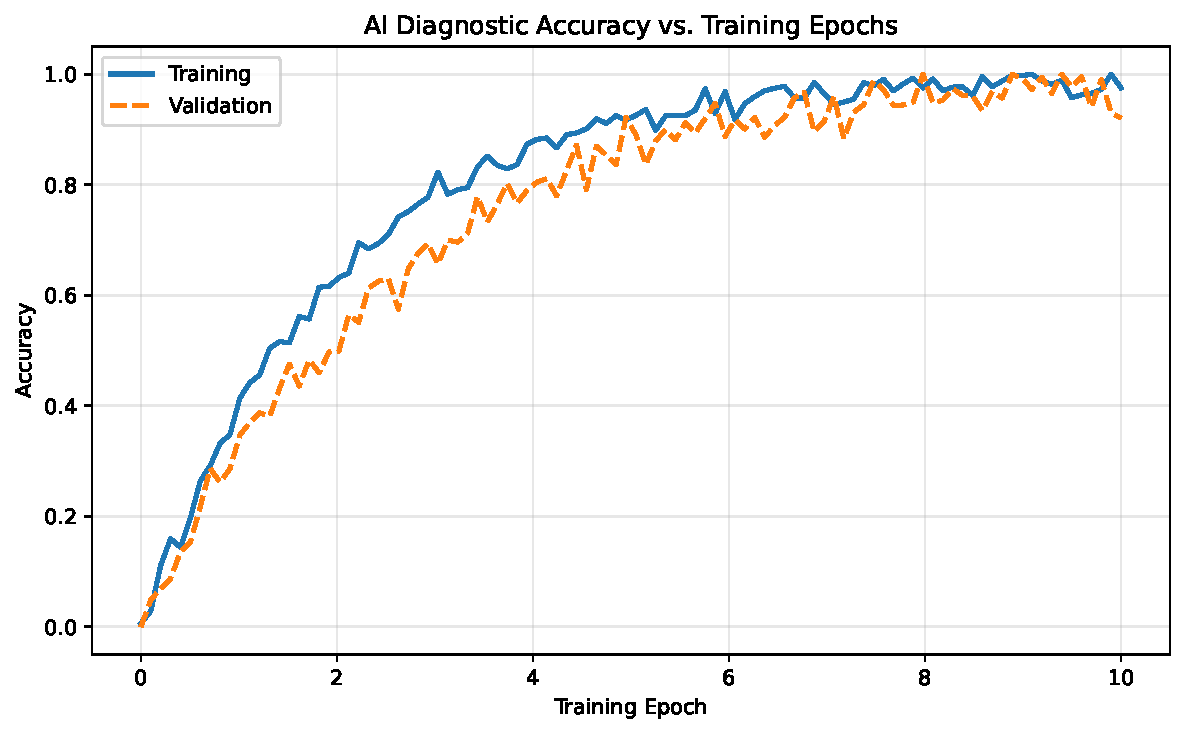
\includegraphics[width=0.88\textwidth]{../assets/graphs/accuracy_curve.pdf}
  \caption{AI diagnostic accuracy as a function of training epochs, generated with Python/matplotlib. Training accuracy (solid) and validation accuracy (dashed) converge as the model generalises to unseen medical data \cite{lecun2015deep}.}
  \label{fig:accuracy_curve}
\end{figure}

\section{Personalized Medicine and Treatment Optimization}
The advent of AI agents is fundamentally transforming personalized medicine, moving healthcare towards highly individualized treatment approaches. By analyzing vast and complex patient data, AI agents can recommend tailored treatments, optimize drug dosages, and suggest preventive strategies that are specific to each individual. This shift promises to improve therapeutic outcomes and minimize adverse effects, marking a significant evolution in patient care \cite{topol2019highperformance}.

Personalized medicine, enabled by AI, considers a patient's unique genetic makeup, environmental factors, and lifestyle choices. This holistic approach allows for interventions that are far more effective than traditional, generalized treatments. The following subsections detail the mechanisms and benefits of AI in this domain.

\subsection{Genomic Data Analysis for Tailored Therapies}
AI agents are adept at analyzing complex genomic data, identifying specific genetic markers that influence disease susceptibility and drug response. This capability allows for the selection of therapies that are most likely to be effective for a particular patient, based on their unique genetic profile \cite{mckinney2020international}. For example, in oncology, AI can help identify specific mutations in a tumor that make it responsive to certain targeted therapies, avoiding ineffective treatments.

By correlating genomic information with clinical outcomes, AI agents can predict how a patient will react to different medications, minimizing trial-and-error approaches. This not only improves treatment efficacy but also reduces the risk of adverse drug reactions. The integration of genomic insights into treatment planning represents a cornerstone of personalized medicine.

\subsection{Optimizing Drug Dosages and Regimens}
One critical application of AI agents in personalized medicine is the optimization of drug dosages and treatment regimens. Traditional dosing often relies on generalized guidelines, which may not be ideal for every patient due to variations in metabolism, body weight, and comorbidities. AI agents can analyze real-time patient data, including physiological responses and drug levels, to recommend precise dosages that maximize efficacy and minimize toxicity \cite{fleming2018artificial}.

This dynamic adjustment of medication is particularly beneficial for drugs with narrow therapeutic windows, where small deviations in dosage can have significant consequences. AI agents can continuously monitor patient parameters and suggest adjustments, ensuring that each patient receives the optimal amount of medication at the right time. This leads to improved patient safety and better therapeutic outcomes.

\subsection{Predictive Analytics for Preventive Strategies}
AI agents utilize predictive analytics to identify individuals at high risk for future health issues, enabling proactive preventive strategies. By analyzing historical health records, demographic data, and lifestyle factors, these agents can forecast the likelihood of developing chronic diseases or experiencing acute events \cite{shah2019artificial}. This allows healthcare providers to intervene early with personalized recommendations for diet, exercise, or lifestyle modifications.

For example, AI models can predict the risk of developing type 2 diabetes or cardiovascular disease, prompting clinicians to offer targeted preventive programs. This shift from reactive treatment to proactive prevention is a hallmark of AI-driven personalized medicine. By empowering patients and providers with foresight, AI agents contribute to long-term health and well-being.

\section{Ethical Considerations of AI Agents in Healthcare}
The integration of AI agents into healthcare, while promising, introduces a complex array of ethical considerations that must be carefully addressed. These concerns span data privacy, algorithmic bias, accountability for errors, and the potential for dehumanization of care. Ensuring that AI technologies are developed and deployed responsibly is paramount to maintaining patient trust and upholding medical ethics \cite{who2021ai}.

Navigating these ethical challenges requires a multi-faceted approach involving policymakers, clinicians, technologists, and patients. Transparency, fairness, and accountability must be embedded into the design and operation of AI agents. This section explores the key ethical dilemmas posed by AI in healthcare.

\subsection{Data Privacy and Security}
AI agents in healthcare rely on access to vast amounts of sensitive patient data, including medical records, genomic information, and real-time physiological measurements. This extensive data usage raises significant concerns regarding privacy and security \cite{nih_ethical_implications}. Protecting this information from breaches, unauthorized access, and misuse is a fundamental ethical imperative. Robust data governance frameworks, encryption, and anonymization techniques are essential to safeguard patient confidentiality.

The potential for re-identification of anonymized data also poses a challenge, requiring continuous vigilance and advanced privacy-preserving technologies. Patients must be assured that their personal health information is handled with the utmost care and used only for legitimate medical purposes. Establishing clear policies for data access, storage, and sharing is critical for building and maintaining trust.

\subsection{Algorithmic Bias and Fairness}
Algorithmic bias is a significant ethical concern, as AI models can inadvertently perpetuate or amplify existing societal biases present in their training data \cite{campanella2019deep}. If training data disproportionately represent certain demographics or contain historical biases, the AI agent may produce inequitable or inaccurate outcomes for underrepresented groups. This can lead to disparities in diagnosis, treatment recommendations, and access to care.

Addressing algorithmic bias requires careful attention to data collection, model design, and continuous monitoring. Developers must ensure that training datasets are diverse and representative, and that algorithms are rigorously tested for fairness across different patient populations. Transparency in algorithmic decision-making is also crucial to identify and mitigate biases effectively.

\subsection{Accountability for Errors and Dehumanization of Care}
The question of accountability becomes complex when AI agents are involved in clinical decision-making or direct patient care. If an AI agent makes an error that leads to patient harm, determining who is responsible—the developer, the clinician, or the institution—is not always straightforward \cite{fda_ai_ml_samd}. Clear legal and ethical frameworks are needed to assign accountability and ensure patient safety.

Furthermore, the increasing reliance on AI agents raises concerns about the potential dehumanization of care. While AI can enhance efficiency, it must not replace the empathetic and personal aspects of human interaction that are central to healthcare. Maintaining a balance between technological efficiency and human compassion is vital to ensure that patients feel heard, understood, and cared for.

\section{Regulatory Frameworks and Oversight}
The rapid advancement of AI agents in healthcare necessitates the development of robust regulatory frameworks to ensure their safety, efficacy, and ethical deployment. Regulatory bodies worldwide are grappling with how to classify, approve, and monitor AI-driven medical devices and software \cite{gov_uk_mhra_roadmap}. These frameworks are crucial for fostering innovation while protecting patients from potential harms.

The unique characteristics of AI, such as its adaptive learning capabilities and opacity, pose distinct challenges for traditional regulatory approaches. A dynamic and adaptive regulatory landscape is required to keep pace with technological evolution. This section examines the current state and future directions of regulatory oversight for AI in healthcare.

\subsection{Classification of AI as Medical Devices}
A primary challenge for regulators is classifying AI software as a medical device. Many AI agents function as Software as a Medical Device (SaMD), which requires specific regulatory pathways distinct from traditional hardware devices \cite{fda_ai_ml_samd}. Regulators must determine the level of risk associated with different AI applications, from low-risk administrative tools to high-risk diagnostic or therapeutic agents. This classification dictates the rigor of pre-market approval processes and post-market surveillance.

The adaptive nature of some AI models, which can continuously learn and evolve post-deployment, further complicates classification. Regulators are exploring approaches that allow for iterative updates while ensuring safety and performance. Clear guidelines on what constitutes a significant change requiring re-approval are essential for developers and healthcare providers.

\subsection{Approval Pathways and Post-Market Surveillance}
Establishing clear approval pathways for AI agents is critical for their timely and safe integration into clinical practice. These pathways typically involve rigorous testing, validation against clinical endpoints, and demonstration of efficacy and safety \cite{regdesk_eu_ai_act}. However, traditional clinical trial designs may not be fully adequate for evaluating AI systems, especially those with continuous learning capabilities. Innovative methodologies, such as real-world evidence generation, are being explored.

Post-market surveillance is equally important to monitor the performance and safety of AI agents once they are deployed. This includes tracking adverse events, identifying performance drifts, and ensuring that algorithms remain fair and unbiased over time. Continuous monitoring mechanisms and reporting requirements are vital for maintaining public trust and ensuring ongoing safety.

\subsection{International Harmonization and Collaboration}
Given the global nature of healthcare and technology, international harmonization of regulatory frameworks for AI agents is highly desirable. Divergent regulations across different countries can create barriers to innovation and hinder the global adoption of beneficial AI technologies \cite{who2021ai}. Collaborative efforts among regulatory bodies, industry stakeholders, and academic experts are essential to develop common standards and best practices.

Initiatives aimed at sharing regulatory experiences, developing common terminology, and establishing mutual recognition agreements can facilitate the responsible global deployment of AI in healthcare. Such collaboration can accelerate the development of safe and effective AI agents while ensuring consistent patient protection across borders. This collective approach is crucial for navigating the complexities of AI regulation.

\section{\texthebrew{שילוב סוכני בינה מלאכותית בתהליכי עבודה קיימים}}
\label{sec:hebrew_bidi_chapter}

\subsection{\texthebrew{השקעה בתשתיות ובטכנולוגיה}}
\label{subsec:hebrew_infrastructure}
\begin{hebrewblock}
שילוב מוצלח של סוכני בינה מלאכותית במערכות בריאות דורש השקעה משמעותית בתשתיות טכנולוגיות. בתי חולים ומרפאות צריכים לשדרג את מערכות המחשוב שלהם כדי לתמוך בכוח העיבוד הנדרש עבור מודלי למידת מכונה עתירי נתונים. זה כולל שרתי ענן, אחסון נתונים מאובטח ויכולות רשת חזקות. ללא תשתית מתאימה, היכולות של סוכני הבינה המלאכותית לא ימומשו במלואן.
\end{hebrewblock}
\begin{englishblock}
Successful integration of AI agents into healthcare systems requires significant investment in technological infrastructure. Hospitals and clinics need to upgrade their computing systems to support the processing power required for data-intensive Machine Learning models. This includes cloud servers, secure data storage, and robust network capabilities. Without adequate infrastructure, the full potential of AI agents cannot be realized.
\end{englishblock}

\subsection{\texthebrew{הכשרת כוח אדם וניהול שינויים}}
\label{subsec:hebrew_training}
\begin{hebrewblock}
הטמעת סוכני בינה מלאכותית מחייבת גם הכשרה מקיפה של כוח האדם הרפואי והאדמיניסטרטיבי. רופאים, אחיות וצוות תמיכה צריכים ללמוד כיצד לתקשר עם סוכני בינה מלאכותית, לפרש את הפלטים שלהם ולשלב אותם בתהליכי קבלת ההחלטות הקליניים. תוכניות הכשרה אלו חיוניות כדי להבטיח אימוץ יעיל ולהפחית התנגדות לשינוי. ניהול שינויים אפקטיבי הוא קריטי להצלחה.
\end{hebrewblock}
\begin{englishblock}
Implementing AI agents also necessitates comprehensive training for medical and administrative staff. Physicians, nurses, and support personnel need to learn how to interact with AI agents, interpret their outputs, and integrate them into clinical decision-making processes. These training programs are essential to ensure effective adoption and reduce resistance to change. Effective change management is critical for success.
\end{englishblock}

\subsection{\texthebrew{אינטגרציה עם מערכות קיימות}}
\label{subsec:hebrew_integration}
\begin{hebrewblock}
שילוב סוכני בינה מלאכותית עם מערכות קיימות, כגון רשומות בריאות אלקטרוניות (EHR) ומערכות מידע בבתי חולים (HIS), הוא אתגר טכני משמעותי. יש להבטיח יכולת פעולה הדדית חלקה כדי שסוכני הבינה המלאכותית יוכלו לגשת לנתונים רלוונטיים ולעדכן אותם בזמן אמת. פיתוח ממשקי API סטנדרטיים ופרוטוקולי תקשורת מאובטחים הם צעדים הכרחיים להשגת אינטגרציה מוצלחת.
\end{hebrewblock}
\begin{englishblock}
Integrating AI agents with existing systems, such as Electronic Health Records (EHR) and Hospital Information Systems (HIS), is a significant technical challenge. Seamless interoperability must be ensured so that AI agents can access and update relevant data in real-time. Developing standardized APIs and secure communication protocols are necessary steps to achieve successful integration.
\end{englishblock}

\subsection{\texthebrew{התמודדות עם אתגרי אבטחת מידע}}
\label{subsec:hebrew_security}
\begin{hebrewblock}
אבטחת מידע היא דאגה מרכזית בעת שילוב סוכני בינה מלאכותית, במיוחד לאור הגישה שלהם לנתוני מטופלים רגישים. יש ליישם פרוטוקולי אבטחה מחמירים, כולל הצפנה, בקרת גישה מבוססת תפקידים וביקורות אבטחה קבועות. בנוסף, יש לפתח מנגנונים לזיהוי ותגובה מהירה לאיומי סייבר כדי להגן על שלמות וסודיות הנתונים.
\end{hebrewblock}
\begin{englishblock}
Data security is a paramount concern when integrating AI agents, especially given their access to sensitive patient data. Strict security protocols must be implemented, including encryption, role-based access control, and regular security audits. Furthermore, mechanisms for rapid detection and response to cyber threats need to be developed to protect data integrity and confidentiality.
\end{englishblock}

\subsection{\texthebrew{הערכה מתמשכת ושיפור ביצועים}}
\label{subsec:hebrew_evaluation}
\begin{hebrewblock}
לאחר הטמעתם, סוכני בינה מלאכותית דורשים הערכה מתמשכת ושיפור ביצועים. יש לנטר באופן קבוע את דיוקם, יעילותם והשפעתם על תוצאות המטופלים. משוב מרופאים ומטופלים, יחד עם ניתוח נתונים, יאפשר זיהוי אזורים לשיפור ועדכון המודלים. תהליך איטרטיבי זה מבטיח שסוכני הבינה המלאכותית יישארו רלוונטיים ויעילים לאורך זמן.
\end{hebrewblock}
\begin{englishblock}
Once implemented, AI agents require continuous evaluation and performance improvement. Their accuracy, efficiency, and impact on patient outcomes must be regularly monitored. Feedback from clinicians and patients, along with data analysis, will enable the identification of areas for improvement and model updates. This iterative process ensures that AI agents remain relevant and effective over time.
\end{englishblock}

\section{Future Developments and Human-AI Collaboration}
The future of AI agents in healthcare is poised for continuous innovation, with developments likely focusing on multi-agent systems, explainable AI (XAI), and seamless human-AI collaboration. These advancements aim to further optimize patient outcomes, enhance operational efficiency, and address some of the current limitations of AI technologies \cite{ibm_watson_health}. The trajectory suggests a move towards more sophisticated, transparent, and integrated AI solutions.

The evolution of AI agents will increasingly emphasize their ability to work synergistically with human clinicians, rather than replacing them. This collaborative paradigm promises to unlock new levels of performance and insight in healthcare. This section explores anticipated future developments and the growing importance of human-AI partnership.

\subsection{Multi-Agent Systems and Orchestration}
Future developments will likely see a greater emphasis on multi-agent systems, where multiple AI agents collaborate to achieve complex goals \cite{davenport2019ai}. For example, one agent might specialize in diagnostic image analysis, another in genomic interpretation, and a third in treatment planning, all coordinating to provide a comprehensive patient assessment. This orchestration of specialized agents can tackle more intricate problems than single-purpose agents alone.

These systems will require advanced coordination mechanisms and communication protocols to ensure seamless data exchange and decision-making. The ability of agents to learn from each other and adapt their strategies dynamically will be crucial. Multi-agent systems promise to enhance the holistic management of patient care, integrating diverse data sources and analytical capabilities.

\subsection{Explainable AI (XAI) for Trust and Transparency}
A critical area of future development is Explainable AI (XAI), which aims to make AI decision-making processes more transparent and understandable to human users \cite{goodfellow2016deep}. Currently, many deep learning models operate as "black boxes," making it difficult to understand why a particular diagnosis or treatment recommendation was made. XAI techniques will provide insights into the reasoning behind AI outputs, fostering greater trust and accountability.

For clinicians, understanding the rationale behind an AI agent's suggestion is essential for informed decision-making and for identifying potential biases or errors. XAI will enable healthcare professionals to validate AI recommendations, integrate them more confidently into their practice, and explain them to patients. This transparency is vital for ethical deployment and widespread adoption.

\subsection{Seamless Human-AI Collaboration}
The ultimate goal of future AI agent development in healthcare is to achieve seamless human-AI collaboration. This involves designing interfaces and interaction models that allow clinicians and AI agents to work together intuitively and effectively \cite{oracle_cloud}. AI agents will act as intelligent assistants, providing real-time insights, automating routine tasks, and augmenting human cognitive abilities, allowing clinicians to focus on complex problem-solving and patient interaction.

This collaboration will extend beyond simple decision support to dynamic partnerships where AI agents adapt to human preferences and learning styles. The future envisions a healthcare ecosystem where AI agents are integrated into every aspect of care, from administrative tasks to complex surgical procedures, all while maintaining a human-centric approach. This synergy promises to elevate the quality, efficiency, and personalization of healthcare delivery.

\section{Challenges and Limitations of AI Agents}
Despite the transformative potential of AI agents in healthcare, their widespread adoption and effective integration face several significant challenges and limitations. These include technical hurdles, ethical dilemmas, regulatory complexities, and practical implementation issues. Addressing these limitations is crucial for realizing the full benefits of AI in medicine while mitigating potential risks.

Recognizing these challenges is the first step towards developing robust solutions and ensuring responsible innovation. The complexities extend beyond mere technological development to encompass societal, organizational, and human factors. This section delves into the primary obstacles hindering the seamless integration of AI agents.

\subsection{Data Quality and Interoperability}
The effectiveness of AI agents heavily relies on the quality, quantity, and accessibility of data. Poor data quality, including incomplete, inconsistent, or biased datasets, can lead to inaccurate or unreliable AI outputs \cite{davenport2019ai}. Furthermore, the lack of interoperability between different healthcare information systems poses a major challenge. Data often resides in fragmented silos, making it difficult for AI agents to access and integrate comprehensive patient information across various platforms and providers.

Achieving true interoperability requires standardized data formats, robust data sharing agreements, and advanced integration technologies. Without these, AI agents cannot leverage the full spectrum of available patient data, limiting their diagnostic and predictive capabilities. Investing in data infrastructure and standardization is paramount for unlocking AI's potential.

\subsection{Resistance to Adoption and Workforce Retraining}
The introduction of AI agents into healthcare workflows can encounter resistance from clinicians and administrative staff. Concerns about job displacement, the perceived threat to professional autonomy, and a lack of understanding of AI capabilities can hinder adoption \cite{topol2019deep}. Overcoming this resistance requires effective change management strategies, clear communication about AI's role as an assistive tool, and demonstrable benefits.

Moreover, the healthcare workforce requires significant retraining to effectively interact with and utilize AI agents. Clinicians need new skills to interpret AI outputs, understand algorithmic limitations, and integrate AI-generated insights into their practice. Educational programs and continuous professional development are essential to prepare the workforce for an AI-augmented future.

\subsection{Cost of Implementation and Maintenance}
The initial cost of implementing AI agent systems in healthcare can be substantial, encompassing hardware, software licenses, data infrastructure, and integration services. Developing and deploying sophisticated AI models requires significant financial investment, which can be a barrier for many healthcare organizations, especially smaller institutions \cite{microsoft_azure_ai}. The ongoing maintenance, updates, and monitoring of AI systems also incur considerable costs.

Beyond initial deployment, AI models require continuous refinement and retraining with new data to maintain their performance and relevance. This necessitates dedicated resources and expertise. Balancing the high costs of implementation and maintenance with the potential long-term benefits and return on investment is a critical consideration for healthcare stakeholders.

\section{Conclusion}
The integration of AI agents into healthcare represents a profound transformation, offering unprecedented opportunities to enhance diagnostic accuracy, personalize treatment, and streamline administrative processes. This article has systematically explored the diverse applications of AI agents, from their foundational technologies in machine learning and natural language processing to their impact on clinical decision support and operational efficiency. The analysis underscores that while AI agents hold immense promise for revolutionizing healthcare, their successful and ethical deployment is contingent upon addressing a complex interplay of challenges.

The central argument of this paper is that the responsible integration of AI agents hinges on robust regulatory frameworks, transparent algorithmic design, and a proactive approach to addressing inherent biases and ensuring patient trust. Key findings highlight the critical need for clear guidelines on data privacy and security, rigorous efforts to mitigate algorithmic bias, and well-defined accountability mechanisms for errors. Furthermore, substantial investments in technological infrastructure, comprehensive workforce retraining, and seamless interoperability between systems are essential for effective implementation. The future trajectory points towards multi-agent systems, explainable AI, and enhanced human-AI collaboration, emphasizing a synergistic partnership that augments human capabilities rather than replacing them. By proactively addressing these multifaceted challenges, healthcare systems can harness the full potential of AI agents to deliver higher quality, more efficient, and truly personalized patient care.

\printbibliography[heading=bibintoc]

\end{document}